\chapter{BrowserAudit as it stands}


\section{Initial project}

Charlie Hothersall's thesis can be found in \cite{charlie} , Browseraudit was built largely as a modification of Mocha with Chai assertion library \
Mocha was meant to be a nodejs testing library, but had browser support, hence allowed to have a base framework to save time and get the actual tests written \

It was really thought of as a Unit Testing framework code running on the browser which was in a way a valid analogy to Unit tests that the browser developers would \
have written for the implementation of security policies for their browsers, but of course here done at the client level. While Mocha helped save some time for the task and
it's asynchronous options were appreciated to save time running the tests; It did however need to be heavily customized with a rebuilt frontend using a Reporter interface that \
triggers callbacks on testStart end and Suite start and End.\ 

The frontend was beautifully done, making use of twitter bootstrap, with suitable design that didn't get in the way of understanding the tests, and that offered expandable\
information about the tests from just the name and category and Pass/fail down to the exact code and the assertions that fail or errors matching different users capabilities.\

There were a fair amount of basic tests of which the most notable one that illustrates an important tool for running these tests which is the img src property:
you can see this in action in \ref{fig:sop} 

\begin{figure}
\centering
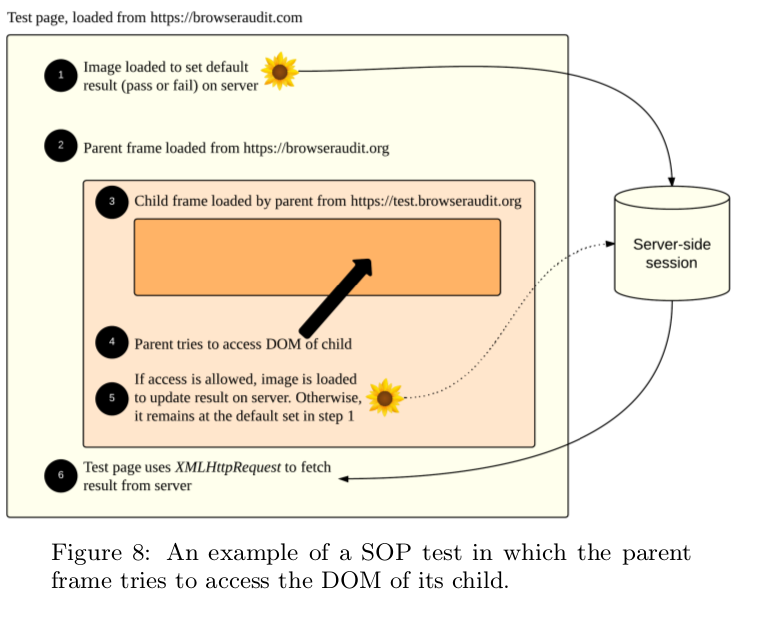
\includegraphics[width=1\textwidth]{./SOPbasic.png}
\caption{\label{fig:sop}Same origin policy typical test}
\end{figure}

As you can see the mechanism of img src property is used to communicate to the server on predefined appropriate pass/fail testiD endpoints. This is because 
the img object is not subject to any limitations and doesn't interfere in the testing of the security policy itself. This is used in many other types of tests.

The initial version had over 300 test tests and by using plain javascript and dilligently avoiding methods that are not adopted by most browsers,
The initial browseraudit version was supported and tested on these browsers:

\begin{itemize}
 \item Firefox desktop version 26, 29 => 4/306 and 6/306 failures respectively
 \item Android version 30 => 14 failures
 \item Ie10 => 74/306 failures issues running the actual tests, the failures are test implementation issues.
 \item Ie11  => 64/306 In this instance some of the tests that failed in ie10 run but they are still failures.
 \item Safari Desktop version 6 and Ios Version => 6 /286 runs fast with few errors, less tests because no HSTS.
 \item Android 4.2.2 => 64/267 problems with CORS and AJAX implementation
 \item Android 4.4.2 => 2/286 failing test due to X-frame-Options ALLOW FROM not implemented.
\end{itemize}

Most notable discoveries of browseraudit were firefox's CSP implementation: CSP allows local CSS @import with only `unsafe-inline' set and 
CSP allows local Worker construction with only `unsafe-inline' set a very good spot that would have been very hard to detect in the wild!

\section{Current version adding tests}

As you can see above  